\begin{figure}[h]
\centering
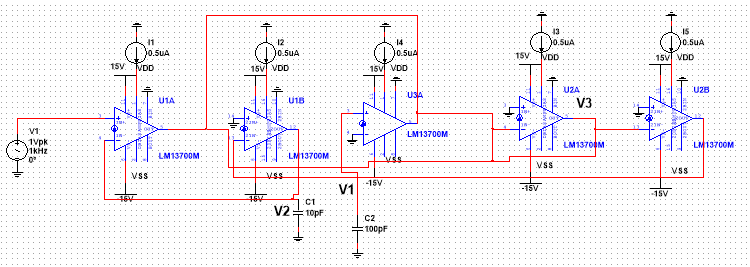
\includegraphics[scale=0.7]{bplphp.png}
\caption{Obecná OTA struktura pro bikvad\label{s:BIK1}}
\end{figure}
\begin{figure}[h]
\centering
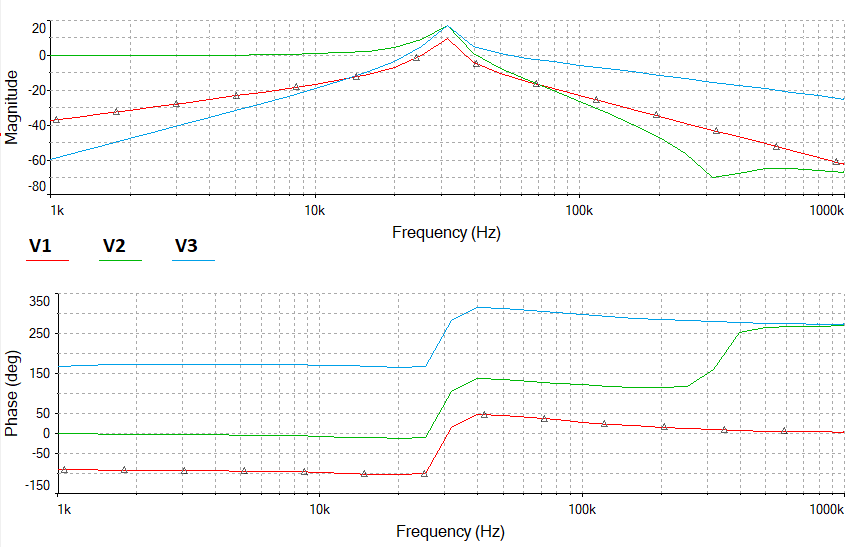
\includegraphics[scale=0.7]{bplphp2.png}
\caption{Amplitudová a fázová charakteristika DP,PP,HP\label{s:BIK2}}
\end{figure}
\begin{figure}[h]
\centering
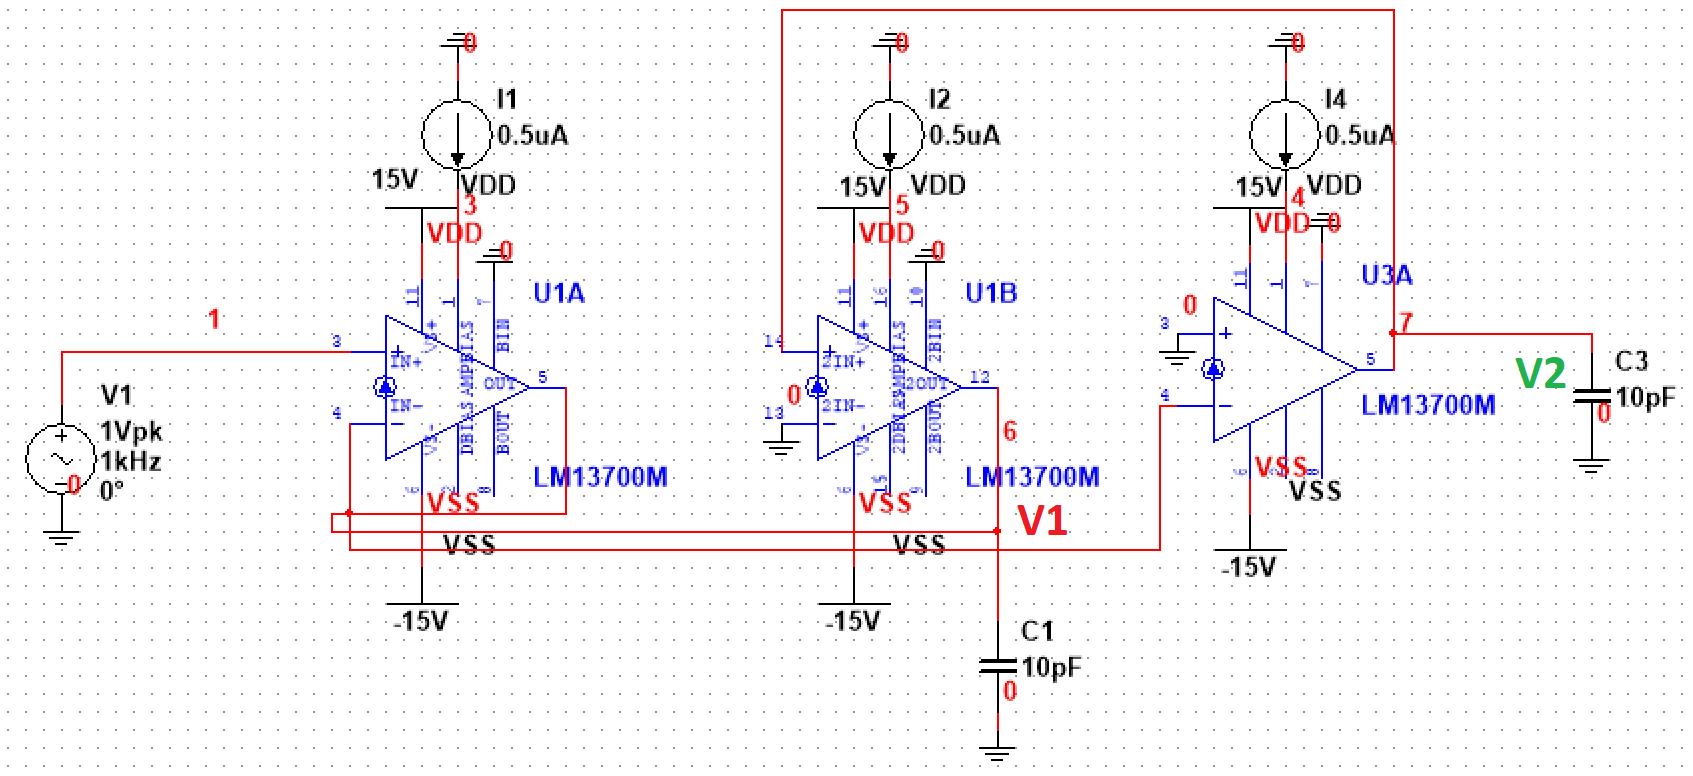
\includegraphics[scale=0.3]{bplp.png}
\caption{Schéma zapojení DP 2. řádu, PP 1. řádu}
\end{figure}
\begin{figure}[h]
\centering
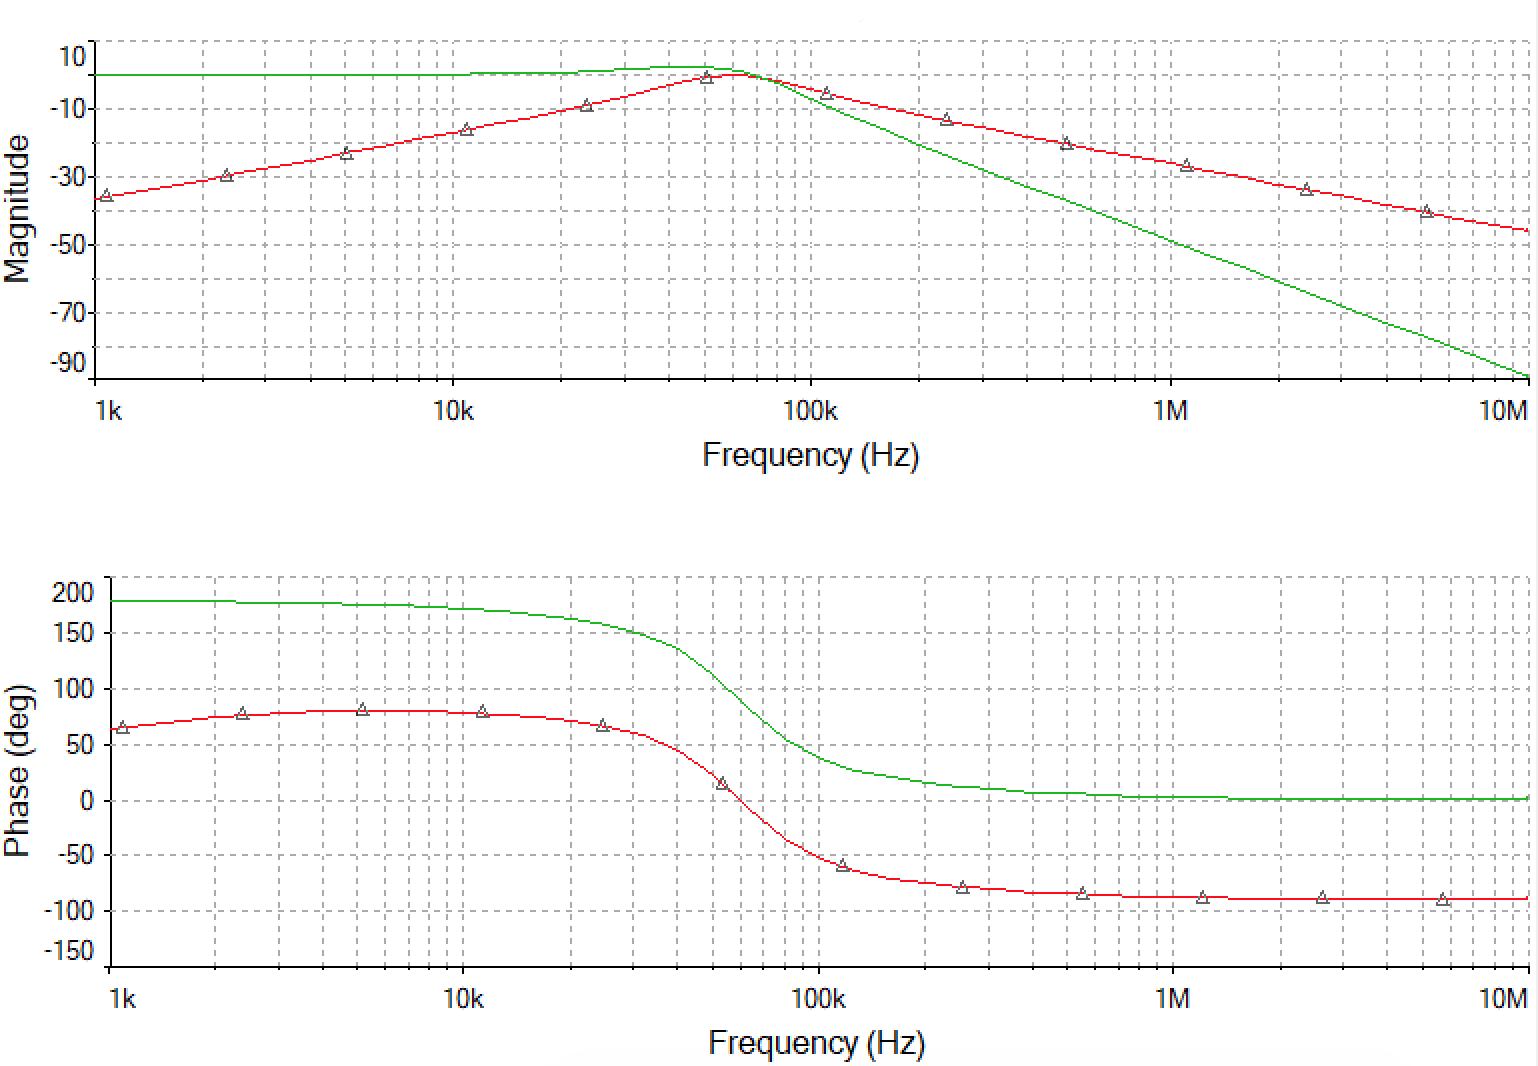
\includegraphics[scale=0.55]{bplp2.png}
\caption{Amplitudová a fázová charakteristika DP 2. řádu, PP 1. řádu\label{s:PET}}
\end{figure}
\begin{figure}[h]
\centering
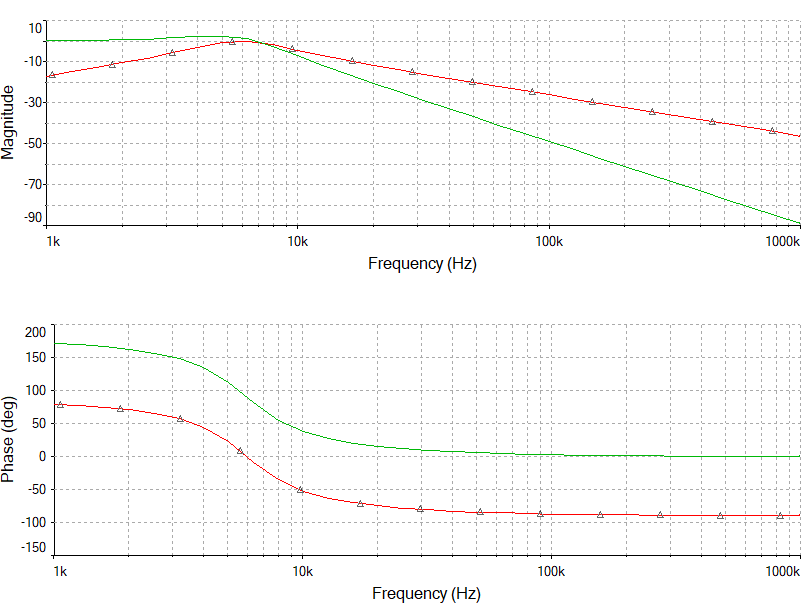
\includegraphics[scale=0.65]{bias.png}
\caption{Amplitudová a fázová charakteristika DP 2. řádu, PP 1. řádu\label{s:PET1}}
\end{figure}
\begin{figure}[h]
\centering
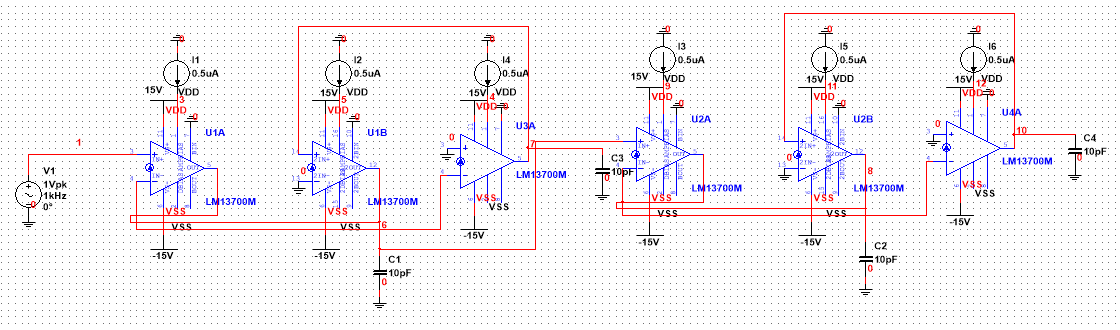
\includegraphics[scale=0.55]{PP2O.png}
\caption{Schéma zapojení DP 4. řádu, PP 2. řádu \label{s:DP4}}
\end{figure}
\begin{figure}[h]
\centering
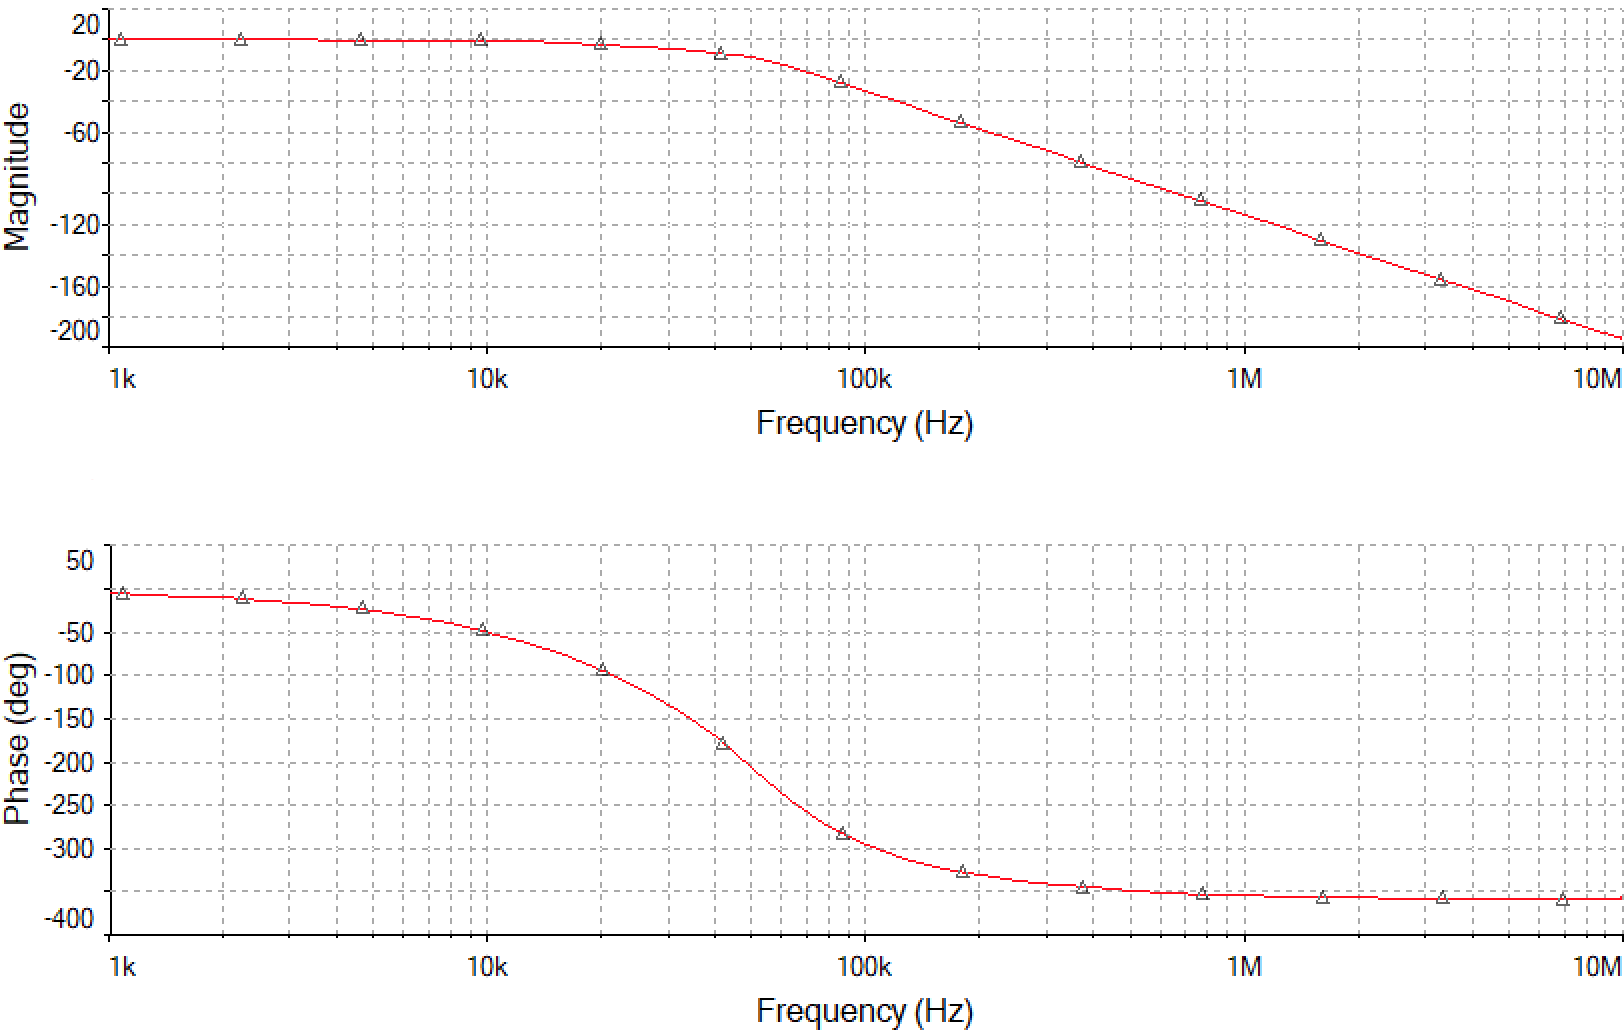
\includegraphics[scale=0.5]{bplp3.png}
\caption{Amplitudová a fázová charakteristika DP 4. řádu}
\end{figure}
\begin{figure}[h]
\centering
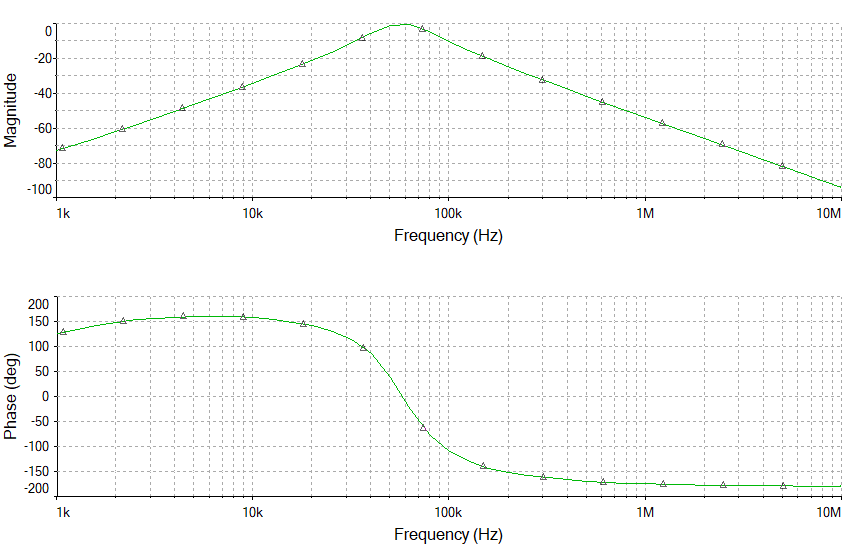
\includegraphics[scale=0.65]{PP2O2.png}
\caption{Amplitudová a fázová charakteristika PP 2. řádu}
\end{figure}
\begin{figure}[h]
\centering
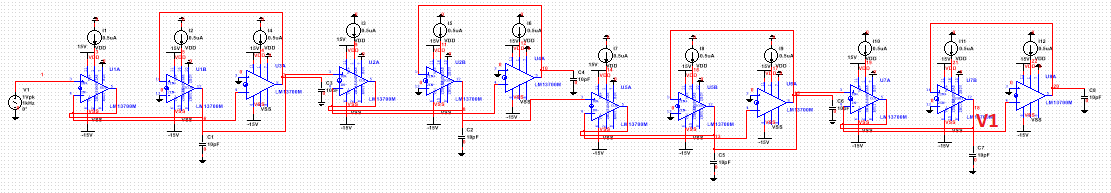
\includegraphics[scale=0.6]{PP4O.png}
\caption{Schéma zapojení PP 4. řádu \label{s:PP4}}
\end{figure}
\begin{figure}[h]
\centering
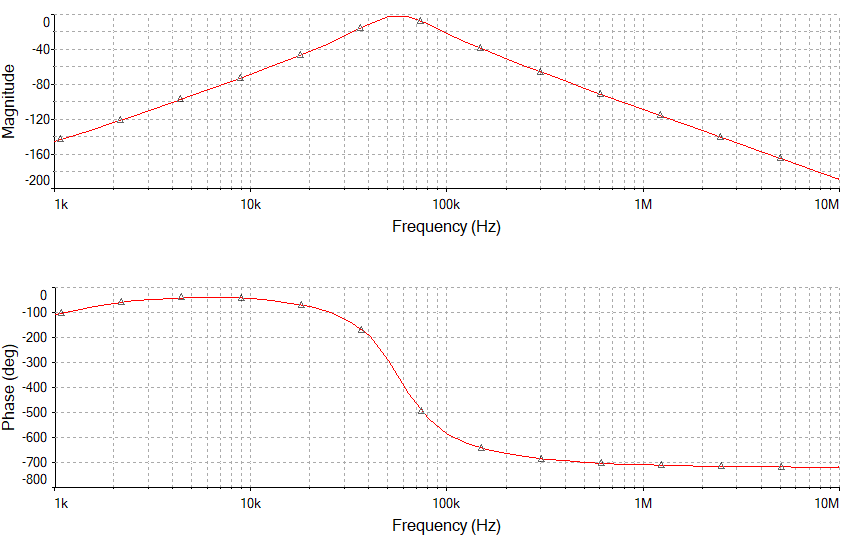
\includegraphics[scale=0.65]{PP4O2.png}
\caption{Amplitudová a fázová charakteristika PP 4. řádu}
\end{figure}
\begin{figure}[h]
\centering
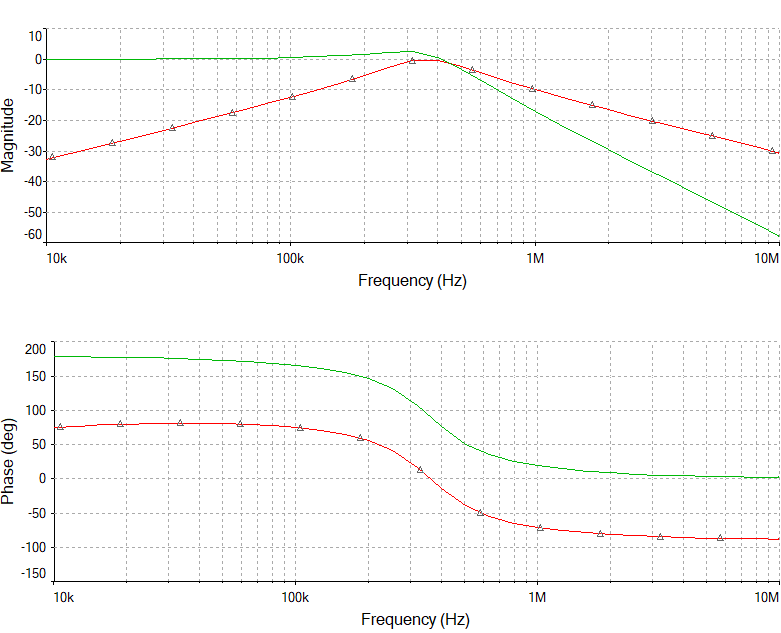
\includegraphics[scale=0.65]{3mikro.png}
\caption{Amplitudová a fázová charakteristika DP 2. řádu, PP 1. řádu \label{s:O1}}
\end{figure}
\begin{figure}[h]
\centering
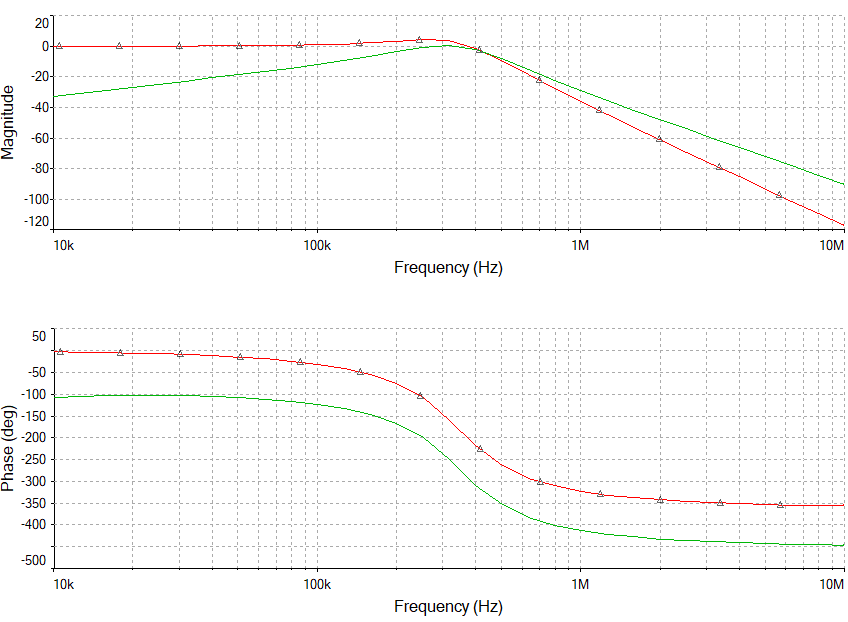
\includegraphics[scale=0.6]{3mikro3.png}
\caption{Amplitudová a fázová charakteristika DP 4. řádu, PP 2. řádu \label{s:O2}}
\end{figure}
\begin{figure}[h]
\centering
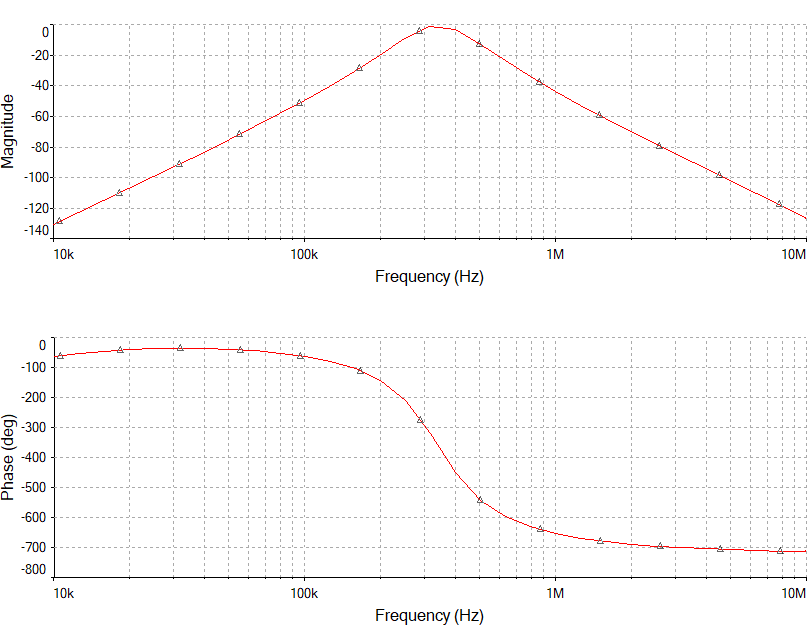
\includegraphics[scale=0.65]{3mikro2.png}
\caption{Amplitudová a fázová charakteristika PP 4. řádu \label{s:O3}}
\end{figure}